\documentclass[12pt]{article}
\setlength{\textwidth}{167mm}
\setlength{\headsep}{0mm}
\setlength{\headheight}{0mm}
\setlength{\textheight}{230mm}
\setlength{\oddsidemargin}{1.6mm}
\setlength{\evensidemargin}{1.6mm}
\setlength{\topmargin}{4.6mm}

\usepackage{chngcntr}
\usepackage{xspace}
\usepackage{graphicx}
\usepackage{amsmath}	% Advanced maths commands
\usepackage{amssymb}	% Extra maths symbols
\usepackage[ ]{hyperref}
\graphicspath{{Images/}}
%\usepackage[symbol]{footmisc}


% Astronomical abbreviations (thanks to Dan Huber)
\newcommand{\numax}{\mbox{$\nu_{\rm max}$}\xspace}
\newcommand{\dnu}{\mbox{$\Delta \nu$}\xspace}
\newcommand{\muHz}{\mbox{$\mu$Hz}\xspace}
\newcommand{\teff}{\mbox{$T_{\rm eff}$}\xspace}
\newcommand{\logg}{\mbox{$\log(g)$}\xspace}
\newcommand{\feh}{\mbox{$\rm{[Fe/H]}$}\xspace}
\newcommand{\msun}{\mbox{$\mathrm{M}_{\odot}$}\xspace}
\newcommand{\lsun}{\mbox{$\mathrm{L}_{\odot}$}\xspace}
\newcommand{\mearth}{\mbox{$\mathrm{M}_{\oplus}$}\xspace}
\newcommand{\rsun}{\mbox{$\mathrm{R}_{\odot}$}\xspace}
\newcommand{\kepler}{\emph{Kepler}\xspace}
\newcommand{\tess}{\emph{TESS}\xspace}
\newcommand{\ktwo}{K2\xspace}
\newcommand{\gaia}{\emph{Gaia}\xspace}

\begin{document}

\section*{\underline{Supplementary Information}}
\tableofcontents

\section{Asteroseismic Model}\label{s:seismo}
In order to extract signatures of stellar rotation from the asteroseismic p mode frequencies, we built a model that simultaneously treats the convective background ($B(\nu)$), the oscillations ($O(\nu)$), and the white noise ($W$), where $\nu$ is frequency \cite{davies+2015}. Our data, observed with \kepler, are also subject to the apodization (attenuation) of signals in the frequency-domain, where we fit our model \cite{chaplin+2011}. The apodization in power is given by

\begin{equation}\label{eq:apodization}
	\eta^2(\nu) = \rm{sinc}^2\left(\frac{\pi}{2}\frac{\nu}{\nu_{\rm nyq}}\right)\, ,
\end{equation}
where $\nu_{\rm nyq}$ is the Nyquist frequency for the \kepler short cadence, which was treated as a free parameter in our model to account for gaps in the data. Apodization only affects signals with characteristic timescales, meaning that it does not affect the white noise level, only the oscillations and convective background components. Given the above, our comprehensive model for the power spectrum is

\begin{equation}\label{eq:model}
	M(\nu) = W + \eta^2(\nu)[O(\nu) + B(\nu)]\, .
\end{equation}

\subsection{Convective Background ($B(\nu)$)}
To model the convective background we used three Harvey components \cite{harvey1985}, which express the background in power as Lorentzian-like functions centered on zero frequency. The Harvey components take the form 

\begin{equation}
	H(\nu, a, b, x) = \frac{4a^2/b}{1 + (2\pi b\nu)^x}\, ,
\end{equation}

\noindent where $a$ and $b$ are the free parameters in our model, and $x$ is fixed. The three Harvey components together form our background function as

\begin{equation}\label{eq:background}
	B(\nu) = H(\nu, a, b, x=4) + H(\nu, c, d, x=4) + H(\nu, j, k, x=2)\, ,
\end{equation}

\noindent where we have labeled parameters for the separate components. The $x = 2$ term here contributes to the background at high frequencies, whereas the $x=4$ terms contribute the background at low frequencies.

\subsection{Modes of Oscillation ($O(\nu)$)}
Modes of oscillation appear in the power spectrum as Lorentzian peaks \cite{chaplin+basu2017}. These peaks can be described by three values: the radial order ($n$, the overtone number of the oscillation), the angular degree ($\ell$) and the azimuthal order ($m$). Due to stellar rotation, each mode with an angular degree of $\ell > 0$ is split into its $(2\ell +1)$ Lorentzian components, labeled by $m$. For all $\ell=(0,1,2)$ modes identified for our targets in the  `Kages'  and LEGACY studies \cite{davies+2016,lund+2017} we add a (set of) Lorentzian(s) to our model, building a composite model representing all visible modes. The construction of our oscillation model takes the form

\begin{equation}
	O(\nu) = \sum_n \sum_\ell \sum_{m=-\ell}^\ell \frac{H_{n,\ell,m}}{1 + \frac{4}{\Gamma^2_{n,\ell}}(\nu - \nu_{n,\ell,m})^2}\, ,
\end{equation}

\noindent where $H_{n,\ell,m}$ is the height of the mode, $\Gamma_{n,\ell}$ is the linewidth of the mode (approximated to be equal for all split azimuthal orders at a single $n$ and $\ell$) and $\nu_{n, \ell, m}$ is the frequency of the mode. The range of $n$ differs per star depending on how many radial orders were reported in LEGACY or Kages, and the range of $\ell$ depends on how many angular degrees were reported for the corresponding radial order.

\subsubsection{Mode Frequencies and Rotational Splitting ($\nu_{n,\ell,m}$)}\label{ssec:frequencies}
The mode frequencies of main sequence stars are described by the asymptotic expression \cite{tassoul1980, vrard+2016}. The asymptotic expression defines the locations of the modes as regularly spaced, with structured deviation around \numax, the frequency of maximum oscillation amplitude. The expression takes the form

\begin{equation}\label{eq:asymptotic}
	\nu_{n,\ell,m} = \dnu\left(n + \epsilon + \delta\nu_{0\ell} + \frac{\alpha}{2}(n - \frac{\numax}{\dnu} + \epsilon)^2\right) + m\nu_{s}\, ,
\end{equation}

\noindent where \dnu is the large frequency separation between two consecutive radial orders $n$, $\epsilon$ is a a phase offset, $\delta\nu_{0\ell}$ is the small frequency separation between two oscillation modes of different $\ell$ at the same radial order, $\alpha$ describes the curvature of the spacing around \numax, and $\nu_s$ is the rotational splitting. Note that here we have expressed the small separation $\delta\nu_{0\ell}$ as a fraction of $\dnu$. In order to improve the computational efficiency of this analysis, we fixed \dnu to the values reported in LEGACY and Kages.

Instead of calculating mode frequencies directly from Equation \ref{eq:asymptotic} for the model, we treated the individual mode frequencies as parameters as well, drawn from Equation \ref{eq:asymptotic}. This is called a `latent parameter' implementation \cite{hogg2012, hall+2019}, as it forms a step between the parameters we want to draw inference on (also called hyperparameters) and our data. 
The parameters $\nu_{n,\ell,m}$ were allowed to vary within an uncertainty $\sigma_{\ell}$, which has a single value for each angular degree and also varied as a free parameter.
This allowed us to account for small shifts in frequency due to sudden changes in the stellar structure \cite{mazumdar+2014}. 

The mode frequency latent parameters were drawn from a normal distribution using Equation \ref{eq:asymptotic} as its mean function, as

\begin{equation}
	\nu_{n, \ell, m} \sim \mathcal{N}(\nu_{n, \ell, m}, \sigma_{\ell})\, ,
\end{equation}

\noindent where the expression $\nu_{n, \ell, m}$ on the right hand side represents the contents of Equation \ref{eq:asymptotic}, and $\mathcal{N}$ represents a normal distribution with a mean equal to $\nu_{n, \ell, m}$ and a standard deviation equal to $\sigma_{\ell}$. The symbol `$\sim$' indicates that the parameters on the left hand side of the equation are drawn from the probability distribution on the right hand side. This notation will be used throughout this work.

\subsubsection{Mode Linewidth ($\Gamma_{n,\ell}$)}
The linewidths of asteroseismic p modes vary roughly as a function of mode frequency, and do so slowly relative to \dnu. This can be expressed as an empirical relation \cite{lund+2017, davies+2014, appourchaux+2016}. However, this relation has six free parameters, none of which are directly relevant to this work. Instead of fitting this relation, we chose to employ a more flexible Gaussian Process \cite[GP]{rasmussen+williams2006} to act as a prior on the linewidths. This can be considered as us modelling the linewidths as correlated measurements, effectively loosely constraining how linewidth varies with frequency.

A GP is defined by a covariance kernel (describing the degree of correlation between linewidths) and a mean function (describing a global trend with frequency). As this approach describes the mode linewidths relative to one another in frequency, the radial orders of each target $n$ were rescaled to be between 0 (for the lowest $n$) and 1 (for the highest $n$)\footnote{The radial orders of $\ell = 2$ modes were increased by $1$ to ensure this approximation applied to all modes.}. This approximation was used to describe the change in linewidth as a function of frequency without depending on the exact frequencies of the modes, which themselves were free parameters (see above). Given this, we defined our GP covariance kernel as a Squared Exponential Kernel to capture the slight periodicity of linewidth with frequency, as

\begin{equation}\label{eq:gpkernel}
	K_{i,j} = \rho^2 \exp \left[ -\frac{(n_{\textrm{f}, i} - n_{\textrm{f}, j})^2}{2L^2} \right]\, ,
\end{equation}

\noindent where $n_{\rm f}$ is the fractional radial order of a given mode and  $K_{i,j}$ represents an element of the covariance matrix $\underline{K}$, describing the covariance between two values of linewidth at different fractional radial orders. The GP kernel has two hyperparameters: $\rho$, which determines the spread of the kernel in linewidth, and $L$, which determines the length scale in terms of $n_{\rm f}$. The length scale $L$ was significantly larger than the large frequency separation (\dnu) in all cases, and so we considered the use of fractional radial orders a valid approximation in this model.

A linear function was used for the mean of the GP, as

\begin{equation}\label{eq:gpmean}
	\mu = m \times n_{\textrm{f}} + c\, ,
\end{equation}
where $m$ and $c$ are the slope and intercept of the line. The linewidth latent parameters were then drawn from the multivariate probability distribution

\begin{equation}\label{eq:gammagp}
	\Gamma \sim \mathcal{N}(\mu, \underline{K})\, ,
\end{equation}

\noindent where $\Gamma$ represents the linewidths of all the modes in the model. The parameters $m$, $c$ and $\rho$ were marginalised over, whereas $L$ was fixed to a pre-determined value.

\subsubsection{Mode Heights and Angle of Inclination ($H_{n,\ell,m}$)}
The height in power of each mode, $H_{n, \ell, m}$, varies not only as a function of distance in frequency from \numax, but also due to observation conditions, such as inclination angle and passband. In our model, we treated $H_{n, \ell, m}$ as a deterministic parameter, as

\begin{equation}\label{eq:height}
	H_{n, \ell, m} =  \varepsilon_{\ell, m}(i) \frac{2 (A_{n, \ell})^2}{\pi \Gamma_{n, \ell}}\, ,
\end{equation}

\noindent where $\varepsilon_{\ell, m}(i)$ modulates the height as a function of inclination angle $i$ (see below), and $A_{n, \ell}$ and $\Gamma_{n, \ell}$ are the mode amplitude and linewidth respectively for a given radial order and angular degree. Instead of modeling and modulating height directly, we instead sampled in amplitude and linewidth. This approach mitigates the correlations between height and linewidth in the sampling process \cite{toutain+appourchaux1994}.

As done above for the mode frequencies and linewidths, the mode amplitudes $A_{n,\ell}$ were also treated as latent parameters drawn from a probability distribution governed by hyperparameters. For this, we used a Gaussian function $G(\nu)$, centered on $\numax$, as

\begin{equation}\label{eq:amplitude}
	G(\nu) = A \times \exp\left[-\frac{(\nu - \numax)^2}{2w^2}\right]\, ,
\end{equation}

\noindent where $A$ is the modes' amplitude at \numax, and $w$ is the width of the Gaussian, both free parameters in our model. 
The mode amplitude latent parameters were then drawn from the probability distribution

\begin{equation}\label{eq:amplitwod}
	A_{n, \ell} \sim \mathcal{N}(G(\nu_{n,\ell}) \times V_\ell, \sigma_{A})\, ,
\end{equation}

\noindent where $V_\ell$ is a free parameter for the mode visibility of different angular degrees, which should be consistent for all \kepler observations. These parameters describe the difference in relative height between modes of different radial order. The mode visibility for $V_0$ is fixed at 1, and $V_{1,2}$ are treated as free parameters. The parameter $\sigma_{A}$, the uncertainty on the distribution, is also a free parameter, and takes the same value for all amplitudes regardless of angular degree.\\

The angle of inclination of a star with respect to Earth changes the net perturbation by a given mode when integrated across the stellar disc, changing the amplitudes of modes of different azimuthal orders. This is a geometric problem, and is expressed by $\varepsilon_{\ell, m}(i)$, which takes the form \cite{gizon+solanki2003}

\begin{equation}\label{eq:legendre}
	\varepsilon_{\ell, m}(i) = \frac{(\ell - |m|)!}{(\ell + |m|)!}\left[P_\ell^{|m|}(\cos(i))\right]^2\, ,
\end{equation}

\noindent where $P_\ell^{|m|}$ are associated Legendre functions. For the first three angular degrees, Equation \ref{eq:legendre} takes the form \cite{handberg+campante2011}

\begin{equation}
	\begin{split}
		\varepsilon_{0,0}(i) &= 1\, ,\\
		\varepsilon_{1,0}(i) &= \cos^2(i)\, ,    \\
		\varepsilon_{1,\pm1}(i) &= \frac{1}{2}\sin^2(i)\, ,\\
		\varepsilon_{2,0}(i) &= \frac{1}{4}(3\cos^2(i) - 1)^2\, ,\\
		\varepsilon_{2,\pm1}(i) &= \frac{3}{8}\sin^2(2i)\, ,\\
		\varepsilon_{2,\pm2}(i) &= \frac{3}{8}\sin^4(i)\, ,
	\end{split}
\end{equation}

\noindent where the sum of available components for a single $\ell$ are normalized to one.

\subsection{Likelihood Function for $M(\nu)$}\label{sec:like}
If data have Gaussian noise in the time domain, they will appear in the frequency domain with noise following a $\chi^2$ distribution with two degrees of freedom \cite[$\chi^2_2$ hereafter]{woodard1984}. The noise properties of $\chi^2_2$ distributed data are multiplicative, and require a specific treatment when fitting a model. As our frequency bins can be approximated to be independent, we used the likelihood function \cite{anderson+1990},

\begin{equation}
	\ln p(\mathcal{P} | M(\nu)) = \sum_{j=0}^{N-1} \left[\ln[M_j(\nu)] + \frac{\mathcal{P}_j}{M_j(\nu)}\right]\, , 
\end{equation}

\noindent where $\mathcal{P}$ is the power spectral density (and thus our data), and $M(\nu)$ represents our model. The subscript $j$ denotes an individual datum, for a total of $N$ data. We have omitted the dependence of the model $M(\nu)$ on its parameters, for clarity. This equation is functionally equivalent to the evaluation of a gamma distribution of the form $\gamma(\mathcal{P} | 1, \beta)$, where $\beta = 1/M(\nu)$, which is the implementation we used in the sampling process.

\subsection{Model preparation and hyperparameter priors}
\subsubsection{Fitting the convective background}\label{sec:background}
Fitting the convective background, apodization and white noise component must be done for the full range of the power spectrum in order to be accurately constrained. However, fitting a single model to the full range of frequencies is computationally inefficient when we are interested in the modes of oscillation, as these occupy a relatively small range of frequencies.

In order to speed up this process, the background was first fit independently to a subset of our data for each star. This subset was created by removing all frequencies within a range $0.1 \times \dnu$ below and above the minimum and maximum mode frequencies reported in LEGACY and Kages. For KIC 3427720 we also removed frequencies in the range $90\, \mu\rm{Hz} < \nu < 400\, \mu{\rm{Hz}}$, where there were large peaks not of asteroseismic origin, skewing the background fit.

For each star the model function (see Eq. \ref{eq:model}) was fit, as

\begin{equation}
	M_{B}(\nu) = W + \eta^2(\nu)B(\nu)\, ,
\end{equation}

\noindent where $B(\nu)$ is the background model described in Equation \ref{eq:background}. The parameter components of our background fit are then $\phi_B = \{\log(a), \log(b), \log(c), \log(d), \log(j), \log(k), W, \nu_{\rm nyq}\}$, where the parameters of the Harvey components were sampled in log space. The model was fit to the background data using \texttt{PyStan} \cite{vanhoey+2013}, run for 10,000 iterations on each star. 

\subsubsection{Obtaining First Guesses and Prior Values}
In order to utilise some of the prior measurements of our targets without using them as hard constraints on our parameters, some of our model equations were fit to LEGACY and `Kages' data to obtain first guesses and mean values on hyperparameter priors.

For first guesses for parameters in the asymptotic expression, we fit Equation \ref{eq:asymptotic}, \textit{not} including the rotational component $m\nu_s$, to the $\ell = (0, 1, 2)$ mode frequencies reported in LEGACY and `Kages' for each star, using their reported uncertainties. This yielded estimates of $\hat{\epsilon}$, $\widehat{\delta\nu}_{01}$, $\widehat{\delta\nu}_{02}$ and $\hat{\alpha}$, where the hat symbol `\, $\widehat{}$\, ' indicates a prior value (e.g. $\hat{\nu}_{\rm max}$ is taken from LEGACY or `Kages'). While not precise, as we did not mitigate any perturbations due to acoustic glitches, these rough results act as functional first guesses and prior mean values. The relation was fit to each star using PyMC3 \cite{salvatier+2016} using 5000 iterations on 4 chains.

To obtain first guesses for the parameters used to set the GP prior on linewidth, we fit a GP constructed as in Equation \ref{eq:gammagp} to the linewidths of the $\ell = 0$ modes reported in LEGACY. Linewidths were not reported for the other angular degrees in LEGACY, but the estimates may be generalised to other $\ell$, as linewidth is a strong function of frequency.  The relation was fit to each star using PyMC3 using 2500 iterations on 4 chains.

Fitting the LEGACY linewidths yielded rough estimates of $\hat{m}$, $\hat{c}$, $\hat{\rho}$ and $L$ for each star. As is noted in Equation \ref{eq:gammagp}, $L$ was fixed to this fit value when fitting our full model to our data. For stars in `Kages', for which no linewidths were reported, we instead fixed these prior values to $\hat{m} = 1$, $\hat{c} = 0.5$, $\hat{\rho} = 0.1$, and the length scale to $L = 0.3$. These values were chosen to reflect those found for the LEGACY stars.

Finally, we obtained prior values for the Gaussian function describing the distribution of mode amplitudes around \numax (Eq. \ref{eq:amplitude}). The mode amplitude of the highest peak in the spectrum was used for $\hat{A}$, which was typically at or near \numax. For the width of the Gaussian we used the empirical function \cite{lund+2017}

\begin{equation}
	\hat{w} = 0.25 \times \hat{\nu}_{\rm max},\, .
\end{equation}

\noindent For the mode visibilities, we used $\hat{V}_1 = 1.2$ and $\hat{V}_2 = 0.7$, which reflect the results for these parameters reported in the LEGACY catalogue.

\subsubsection{Priors on our Hyperparameters}
Given our first guesses and measured prior values, we can define the prior probabilities of the hyperparameters on which our model depends. For the mode frequency hyperparameters (Eq. \ref{eq:asymptotic}), these are

\begin{equation}
	\begin{split}
		\numax &\sim \mathcal{N}(\hat{\nu}_{\rm max}, 10)\, ,\\
		\epsilon &\sim \mathcal{N}(\hat{\epsilon}, 1)\, ,\\
		\alpha &\sim \ln\mathcal{N}(\ln(\hat{\alpha}), 0.01)\, ,\\
		\delta\nu_{01} &\sim \ln\mathcal{N}(\ln(\widehat{\delta\nu}_{01}), 0.1)\, ,\\
		\delta\nu_{02} &\sim \ln\mathcal{N}(\ln(\widehat{\delta\nu}_{02}), 0.1)\, ,\\
		\sigma_{0,1,2} &\sim \mathcal{C}_{1/2}(\beta = 2)\, ,
	\end{split}
\end{equation}

\noindent where $\ln\mathcal{N}$ represents a log-Normal distribution and $\mathcal{C}_{1/2}$ represents a half-Cauchy distribution\footnote{The half-Cauchy distribution ensures the standard deviations do not inflate to large numbers, and is generally well-behaved close to zero in the case of stars with little deviation from Eq. \ref{eq:asymptotic} \cite{gelman2006}.}, and other symbols are as described above. All three hyperparameters $\sigma_{0,1,2}$ describing the uncertainty on the latent parameters of different angular degree were subject to the same prior.

For the mode linewidths (Eq. \ref{eq:gpkernel} and \ref{eq:gpmean}), our hyperparameter priors took the form

\begin{equation}
	\begin{split}
		m &\sim \mathcal{N}(\hat{m}, 1)\, ,\\
		c &\sim \mathcal{N}(\hat{c}, 1)\, ,\\
		\rho &\sim \ln\mathcal{N}(\ln(\hat{\rho}), 0.1)\, ,\\
	\end{split}
\end{equation}

\noindent where the conventions are the same as above. For our mode amplitudes (Eq. \ref{eq:amplitude} and \ref{eq:amplitwod}), they took the form

\begin{equation}
	\begin{split}
		w &\sim \ln\mathcal{N}(\ln(\hat{w}), 10)\, ,\\
		A &\sim \ln\mathcal{N}(\ln(\hat{A}), 1)\, ,\\
		V_1 &\sim \ln\mathcal{N}(\ln(\hat{V}_1), 0.1)\, ,\\
		V_2 &\sim \ln\mathcal{N}(\ln(\hat{V}_2), 0.1)\, ,\\
		\sigma_A &\sim \mathcal{C}_{1/2}(\beta = 1)\, .
	\end{split}
\end{equation}

As the convective background had already been fit to our data excluding the region where the modes are present, the results from that fit could be used as extremely informative priors on our fit to the region containing the modes, where there is little information present to constrain the background. To do so, we modeled the background parameters $\phi_B$ in our full model as being drawn from a multivariate normal distribution as

\begin{equation}
	\phi_{B}\sim\mathcal{N}(\hat{\phi}_{B},\underline{\Sigma}_{\hat{\phi}_{B}})\, ,
\end{equation}

\noindent where $\hat{\phi}_B$ are the median values of our posterior distributions from our prior background fit, and $\underline{\Sigma}_{\hat{\phi}_{B}}$ is the full covariance matrix of all the posterior distributions from our prior background fit, taking into account the correlations between the different Harvey components.

Finally, we defined the priors on the rotational parameters: the mode splitting ($\nu_s$), and the inclination angle ($i$). In order to give these an appropriate treatment, we made two reparameterizations. First, we sampled the projected rotational splitting, $\nu_{\rm{s}}\sin(i)$, which is more efficiently sampled due to the strong correlations between $i$ and $\nu_{\rm s}$ \cite{ballot+2006,ballot+2008a}. A prior was applied over this as

\begin{equation}
	\nu_s\sin(i) \sim \ln\mathcal{N}(\ln(0.75), 0.75)\, ,
\end{equation}

\noindent where conventions are as above. This subjective prior was chosen to reflect that most stars will have a solar-like rotation, with a long tail to allow for the fastest rotators. Second, we sampled in $\cos(i)$, and gave this a prior of

\begin{equation}
	\begin{split}
		\cos(i) &\sim \mathcal{U}(0, 1)\, ,
	\end{split}
\end{equation}
which is equivalent to stating that probability to observe an inclination angle $i$ is equal to $\sin(i)$. Here, the $\mathcal{U}(0,1)$ indicates a uniform prior between 0 and 1. Using a uniform prior on $\cos(i)$ allowed us to account for the geometric effect that stars with a large inclination angle with respect to us are more common \cite{chaplin+basu2017}.

 \begin{figure*}
	\centering
	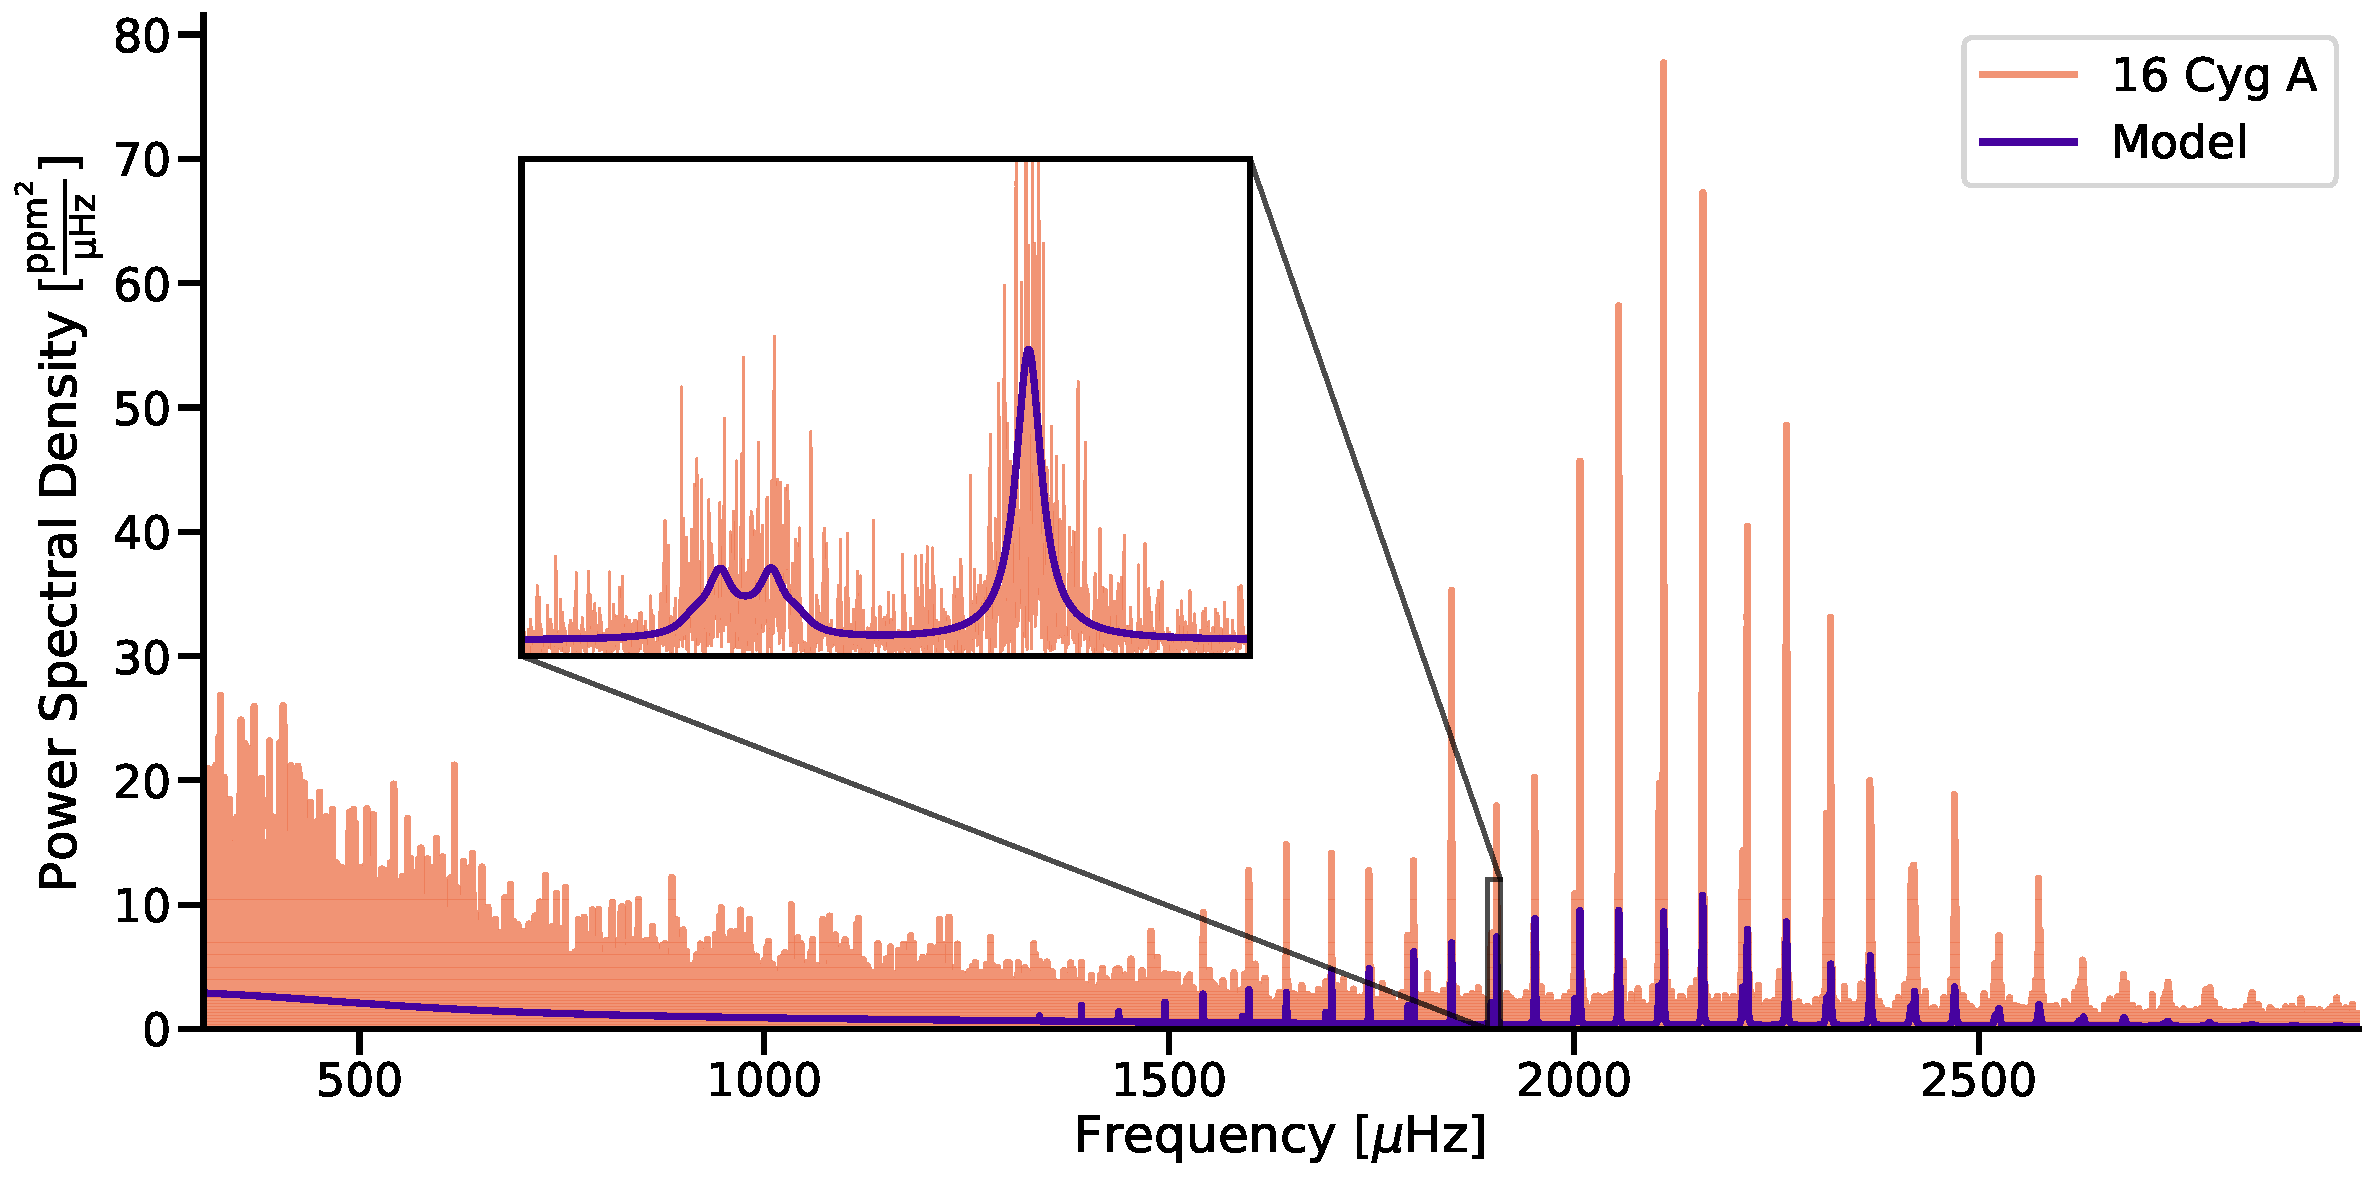
\includegraphics[width=.99\textwidth]{Images/modelfit.pdf}
	\caption{A power spectrum constructed from four years of \kepler observations of 16 Cyg A (KIC 12069424). Plotted over the top is the model resulting from the fit to the data described in this work. The model implements both the mode frequencies, seen on the right hand side of the plot, and the convective background, the effects of which are seen on the left. Low frequencies have been cropped out for clarity. \textit{Inset}: A zoom in on a radial (right) and quadrupole (left) ($\ell = 0, 2$) pair of modes. The quadrupole mode is split into five components by the star's rotation. Due to the star's inclination angle with respect to us, two out of five peaks are more distinct. The height and spacing of the mode components is a function of the star's rotational splitting ($0.56\, \mu\rm{Hz}$, equivalent to $P = 20.5\, \rm{days}$) and angle of inclination ($45^\circ$).}
	\label{fig:modelfit}
\end{figure*}


\subsection{Fitting procedure}
Using our prior information and model described above, we fit Equation \ref{eq:model} to our data $\mathcal{P}$, using the likelihood function described in Section \ref{sec:like}.

In order to speed up the fitting process, we only applied our model to the region of the power spectrum that contains visible modes of oscillation. We created this subset by removing all frequencies outside a range $0.25 \times \Delta\nu$ below and above the minimum and maximum mode frequencies reported in LEGACY and Kages. This region overlaps minimally with the data used to fit for our prior information of the convective background (see Section \ref{sec:background}), so that both model fits are independent.

To improve computational efficiency, we reduced the number of oscillation modes being fit in five targets. For 16 Cyg A \& B, KIC 7970740 and KIC 8478994, we excluded any modes with a Bayes Factor ($\ln(K)$) of less than 6, as reported in LEGACY \cite{davies+2016,lund+2017,kass+raftery1995}. For KIC 8478994, which is reported without a value for $\ln(K)$ in Kages, we only included modes of an overtone number that contained a detection for all of $\ell = (0, 1, 2)$, retaining 5 sets of higher signal-to-noise overtones. We do not expect this reduced scope to bias our results, although they may reduce the precision on our measured rotation rates.

We fit our model to our power spectrum data with \texttt{PyMC3}, using 2500 iterations each on 4 chains. An example of our model fit to an asteroseismic power spectrum of 16 Cyg A is shown in Figure \ref{fig:modelfit}.

\begin{thebibliography}{10}
	\expandafter\ifx\csname url\endcsname\relax
	\def\url#1{\texttt{#1}}\fi
	\expandafter\ifx\csname urlprefix\endcsname\relax\def\urlprefix{URL }\fi
	\providecommand{\bibinfo}[2]{#2}
	\providecommand{\eprint}[2][]{\url{#2}}
	
	\bibitem{davies+2015}
	\bibinfo{author}{Davies, G.~R.} \emph{et~al.}
	\newblock \bibinfo{title}{Asteroseismic inference on rotation, gyrochronology
		and planetary system dynamics of 16 {{Cygni}}}.
	\newblock \emph{\bibinfo{journal}{Monthly Notices of the Royal Astronomical
			Society}} \textbf{\bibinfo{volume}{446}}, \bibinfo{pages}{2959}
	(\bibinfo{year}{2015}).
	
	\bibitem{chaplin+2011}
	\bibinfo{author}{Chaplin, W.~J.} \emph{et~al.}
	\newblock \bibinfo{title}{Ensemble {{Asteroseismology}} of {{Solar}}-{{Type
				Stars}} with the {{NASA Kepler Mission}}}.
	\newblock \emph{\bibinfo{journal}{Science}} \textbf{\bibinfo{volume}{332}},
	\bibinfo{pages}{213} (\bibinfo{year}{2011}).
	
	\bibitem{harvey1985}
	\bibinfo{author}{Harvey, J.}
	\newblock \bibinfo{title}{High-{{Resolution Helioseismology}}}.
	\newblock \emph{\bibinfo{journal}{Future Missions in Solar, Heliospheric \&
			Space Plasma Physics}} \textbf{\bibinfo{volume}{235}}, \bibinfo{pages}{199}
	(\bibinfo{year}{1985}).
	
	\bibitem{chaplin+basu2017}
	\bibinfo{author}{Chaplin, W.~J.} \& \bibinfo{author}{Basu}.
	\newblock \emph{\bibinfo{title}{Asteroseismic {{Data Analysis}}:
			{{Foundations}} and {{Techniques}}}} (\bibinfo{publisher}{{Princeton
			University Press}}, \bibinfo{address}{{Princeton, New Jersey}},
	\bibinfo{year}{2017}), \bibinfo{edition}{1st} edn.
	
	\bibitem{davies+2016}
	\bibinfo{author}{Davies, G.~R.} \emph{et~al.}
	\newblock \bibinfo{title}{Oscillation frequencies for 35 {{Kepler}} solar-type
		planet-hosting stars using {{Bayesian}} techniques and machine learning}.
	\newblock \emph{\bibinfo{journal}{Monthly Notices of the Royal Astronomical
			Society}} \textbf{\bibinfo{volume}{456}}, \bibinfo{pages}{2183}
	(\bibinfo{year}{2016}).
	
	\bibitem{lund+2017}
	\bibinfo{author}{Lund, M.~N.} \emph{et~al.}
	\newblock \bibinfo{title}{Standing on the {{Shoulders}} of {{Dwarfs}}: The
		{{Kepler Asteroseismic LEGACY Sample}}. {{I}}. {{Oscillation Mode
				Parameters}}}.
	\newblock \emph{\bibinfo{journal}{The Astrophysical Journal}}
	\textbf{\bibinfo{volume}{835}}, \bibinfo{pages}{172} (\bibinfo{year}{2017}).
	
	\bibitem{tassoul1980}
	\bibinfo{author}{Tassoul, M.}
	\newblock \bibinfo{title}{Asymptotic approximations for stellar nonradial
		pulsations}.
	\newblock \emph{\bibinfo{journal}{The Astrophysical Journal Supplement Series}}
	\textbf{\bibinfo{volume}{43}}, \bibinfo{pages}{469} (\bibinfo{year}{1980}).
	
	\bibitem{vrard+2016}
	\bibinfo{author}{Vrard, M.}, \bibinfo{author}{Mosser, B.} \&
	\bibinfo{author}{Samadi, R.}
	\newblock \bibinfo{title}{Period spacings in red giants. {{II}}. {{Automated}}
		measurement}.
	\newblock \emph{\bibinfo{journal}{Astronomy and Astrophysics}}
	\textbf{\bibinfo{volume}{588}}, \bibinfo{pages}{A87} (\bibinfo{year}{2016}).
	
	\bibitem{hogg2012}
	\bibinfo{author}{Hogg, D.~W.}
	\newblock \bibinfo{title}{Data analysis recipes: {{Probability}} calculus for
		inference}.
	\newblock \emph{\bibinfo{journal}{arXiv e-prints}}
	\bibinfo{pages}{arXiv:1205.4446} (\bibinfo{year}{2012}).
	
	\bibitem{hall+2019}
	\bibinfo{author}{Hall, O.~J.} \emph{et~al.}
	\newblock \bibinfo{title}{Testing asteroseismology with {{Gaia DR2}}:
		{{Hierarchical}} models of the {{Red Clump}}}.
	\newblock \emph{\bibinfo{journal}{Monthly Notices of the Royal Astronomical
			Society}} \textbf{\bibinfo{volume}{486}}, \bibinfo{pages}{3569--3585}
	(\bibinfo{year}{2019}).
	\newblock \eprint{1904.07919}.
	
	\bibitem{mazumdar+2014}
	\bibinfo{author}{Mazumdar, A.} \emph{et~al.}
	\newblock \bibinfo{title}{Measurement of acoustic glitches in solar-type stars
		from oscillation frequencies observed by {{Kepler}}}.
	\newblock \emph{\bibinfo{journal}{The Astrophysical Journal}}
	\textbf{\bibinfo{volume}{782}}, \bibinfo{pages}{18} (\bibinfo{year}{2014}).
	\newblock \eprint{1312.4907}.
	
	\bibitem{davies+2014}
	\bibinfo{author}{Davies, G.~R.}, \bibinfo{author}{Chaplin, W.~J.},
	\bibinfo{author}{Elsworth, Y.} \& \bibinfo{author}{Hale, S.~J.}
	\newblock \bibinfo{title}{{{BiSON}} data preparation: A correction for
		differential extinction and the weighted averaging of contemporaneous data}.
	\newblock \emph{\bibinfo{journal}{Monthly Notices of the Royal Astronomical
			Society}} \textbf{\bibinfo{volume}{441}}, \bibinfo{pages}{3009--3017}
	(\bibinfo{year}{2014}).
	
	\bibitem{appourchaux+2016}
	\bibinfo{author}{Appourchaux, T.} \emph{et~al.}
	\newblock \bibinfo{title}{Oscillation mode linewidths and heights of 23
		main-sequence stars observed by {{{\emph{Kepler}}}}
		{\emph{(}}{{{\emph{Corrigendum}}}}{\emph{)}}}.
	\newblock \emph{\bibinfo{journal}{Astronomy \& Astrophysics}}
	\textbf{\bibinfo{volume}{595}}, \bibinfo{pages}{C2} (\bibinfo{year}{2016}).
	
	\bibitem{rasmussen+williams2006}
	\bibinfo{author}{Rasmussen, C.~E.} \& \bibinfo{author}{Williams, C. K.~I.}
	\newblock \emph{\bibinfo{title}{Gaussian Processes for Machine Learning}}.
	\newblock Adaptive Computation and Machine Learning (\bibinfo{publisher}{{MIT
			Press}}, \bibinfo{address}{{Cambridge, Mass}}, \bibinfo{year}{2006}).
	
	\bibitem{toutain+appourchaux1994}
	\bibinfo{author}{Toutain, T.} \& \bibinfo{author}{Appourchaux, T.}
	\newblock \bibinfo{title}{Maximum likelihood estimators: {{An}} application to
		the estimation of the precision of helioseismic measurements}.
	\newblock \emph{\bibinfo{journal}{Astronomy and Astrophysics}}
	\textbf{\bibinfo{volume}{289}}, \bibinfo{pages}{649--658}
	(\bibinfo{year}{1994}).
	
	\bibitem{gizon+solanki2003}
	\bibinfo{author}{Gizon, L.} \& \bibinfo{author}{Solanki, S.~K.}
	\newblock \bibinfo{title}{Determining the {{Inclination}} of the {{Rotation
				Axis}} of a {{Sun}}-like {{Star}}}.
	\newblock \emph{\bibinfo{journal}{The Astrophysical Journal}}
	\textbf{\bibinfo{volume}{589}}, \bibinfo{pages}{1009} (\bibinfo{year}{2003}).
	
	\bibitem{handberg+campante2011}
	\bibinfo{author}{Handberg, R.} \& \bibinfo{author}{Campante, T.~L.}
	\newblock \bibinfo{title}{Bayesian peak-bagging of solar-like oscillators using
		{{MCMC}}: A comprehensive guide}.
	\newblock \emph{\bibinfo{journal}{Astronomy and Astrophysics}}
	\textbf{\bibinfo{volume}{527}}, \bibinfo{pages}{A56} (\bibinfo{year}{2011}).
	
	\bibitem{woodard1984}
	\bibinfo{author}{Woodard, M.~F.}
	\newblock \emph{\bibinfo{title}{Short-{{Period Oscillations}} in the {{Total
					Solar Irradiance}}.}}
	\newblock Ph.D. thesis (\bibinfo{year}{1984}).
	
	\bibitem{anderson+1990}
	\bibinfo{author}{Anderson, E.~R.}, \bibinfo{author}{Duvall, T.~L.} \&
	\bibinfo{author}{Jefferies, S.~M.}
	\newblock \bibinfo{title}{Modeling of {{Solar Oscillation Power Spectra}}}.
	\newblock \emph{\bibinfo{journal}{The Astrophysical Journal}}
	\textbf{\bibinfo{volume}{364}}, \bibinfo{pages}{699} (\bibinfo{year}{1990}).
	
	\bibitem{vanhoey+2013}
	\bibinfo{author}{Van~Hoey, S.}, \bibinfo{author}{{van der Kwast}, J.},
	\bibinfo{author}{Nopens, I.} \& \bibinfo{author}{Seuntjens, P.}
	\newblock \bibinfo{title}{Python package for model {{STructure ANalysis}}
		({{pySTAN}})}.
	\newblock \emph{\bibinfo{journal}{EGU General Assembly Conference Abstracts}}
	\textbf{\bibinfo{volume}{15}}, \bibinfo{pages}{EGU2013--10059}
	(\bibinfo{year}{2013}).
	
	\bibitem{salvatier+2016}
	\bibinfo{author}{Salvatier, J.}, \bibinfo{author}{Wiecki, T.~V.} \&
	\bibinfo{author}{Fonnesbeck, C.}
	\newblock \bibinfo{title}{Probabilistic programming in {{Python}} using
		{{PyMC3}}}.
	\newblock \emph{\bibinfo{journal}{PeerJ Computer Science}}
	\textbf{\bibinfo{volume}{2}}, \bibinfo{pages}{e55} (\bibinfo{year}{2016}).
	
	\bibitem{gelman2006}
	\bibinfo{author}{Gelman, A.}
	\newblock \bibinfo{title}{Prior distributions for variance parameters in
		hierarchical models (comment on article by {{Browne}} and {{Draper}})}.
	\newblock \emph{\bibinfo{journal}{Bayesian Analysis}}
	\textbf{\bibinfo{volume}{1}}, \bibinfo{pages}{515--534}
	(\bibinfo{year}{2006}).
	
	\bibitem{ballot+2006}
	\bibinfo{author}{Ballot, J.}, \bibinfo{author}{Garcia, R.~A.} \&
	\bibinfo{author}{Lambert, P.}
	\newblock \bibinfo{title}{Rotation speed and stellar axis inclination from p
		modes: How {{CoRoT}} would see other suns}.
	\newblock \emph{\bibinfo{journal}{Monthly Notices of the Royal Astronomical
			Society}} \textbf{\bibinfo{volume}{369}}, \bibinfo{pages}{1281--1286}
	(\bibinfo{year}{2006}).
	
	\bibitem{ballot+2008a}
	\bibinfo{author}{Ballot, J.}, \bibinfo{author}{Appourchaux, T.},
	\bibinfo{author}{Toutain, T.} \& \bibinfo{author}{Guittet, M.}
	\newblock \bibinfo{title}{On deriving p-mode parameters for inclined solar-like
		stars}.
	\newblock \emph{\bibinfo{journal}{Astronomy \& Astrophysics}}
	\textbf{\bibinfo{volume}{486}}, \bibinfo{pages}{867--875}
	(\bibinfo{year}{2008}).
	\newblock \eprint{0803.0885}.
	
	\bibitem{kass+raftery1995}
	\bibinfo{author}{Kass, R.~E.} \& \bibinfo{author}{Raftery, A.~E.}
	\newblock \bibinfo{title}{Bayes {{Factors}}}.
	\newblock \emph{\bibinfo{journal}{Journal of the American Statistical
			Association}} \textbf{\bibinfo{volume}{90}}, \bibinfo{pages}{773--795}
	(\bibinfo{year}{1995}).
	
\end{thebibliography}


\end{document}